\section{Так квинтовый или квартовый? Квинто-квартовый круг}
\label{ch:harmony:kvinto-kvarto-round}

На самом деле полное название этого полезного помошника, которго легко сделать из бумаги: <<квинто-квартовый круг мажорных и минорных тональностей>>. Выглядит он странно: см. рисунок \ref{TODO}. И хотелось бы не только научиться им пользоваться, но и понять почему он именно такой.

TODO рисунок

Круг может помочь, если вы хотите:
\begin{itemize}
    \item Подобрать <<сочетающиеся>> аккорды для аккомпанемента песен.
    
    \item Определить, какие ноты входят в ту или иную мажорную или минорную тональность.
    
    \item Сменить <<тональность>> аккомпанемента песни. Человеческим языком: \emph{каждую} ноту исходной тональности нужно повысить или понизить на заданное количество полутонов. Зачем? Чтобы было удобнее петь. При этом интервальная структура (т.е. характер, например, веселый или грустный) музыки не изменится, а произведение <<в целом>> будет звучать ниже или выше, <<подстраиваясь>> таким образом под голос исполнителя.    

    \item Решить <<академические>> задачки, например, определить тональность произведения по нотам или определить параллельную тональность.
    
    \item И много чего ещё\ldots
\end{itemize}

Мы не будем сейчас учиться как решать эти задачки, мы начнем разбираться с устройством круга. А в процессе станет понятно не только, как решать эти задачки, но и многое другое.

Глядя на рисунок \ref{fig:harmony:interval:octave-kon-dis} можно увидеть, что для отдельно взятого звука в пределах октавы существует лишь \emph{два} звука, образующий с исходным звуком совершенный консонанс. Относительно исходного эти звуки находятся на расстоянии в 5 (кварта) и 7 (квинта) полутонов. Оказывается, что можно переупорядочить ноты так, чтобы совершенные консонансы стали соседями исходного звука: один справа, другой слева!

Начнём, например с ноты ДО, и отступая по семь полутонов по часовой стрелке:
\[
    C\rightarrow 
    G\rightarrow 
    D\rightarrow 
    A\rightarrow 
    E\rightarrow 
    B\rightarrow 
    {F\sharp}\rightarrow
    {C\sharp}\rightarrow
    {G\sharp}\rightarrow
    {D\sharp}\rightarrow
    {A\sharp}\rightarrow
    F\rightarrow 
    C
\]
замкнем круг и получим результат, представленный на рисунке \ref{fig:harmony:kvinto-kvarto:kons-rearrange}.

\begin{figure}[!ht]
    \centering
    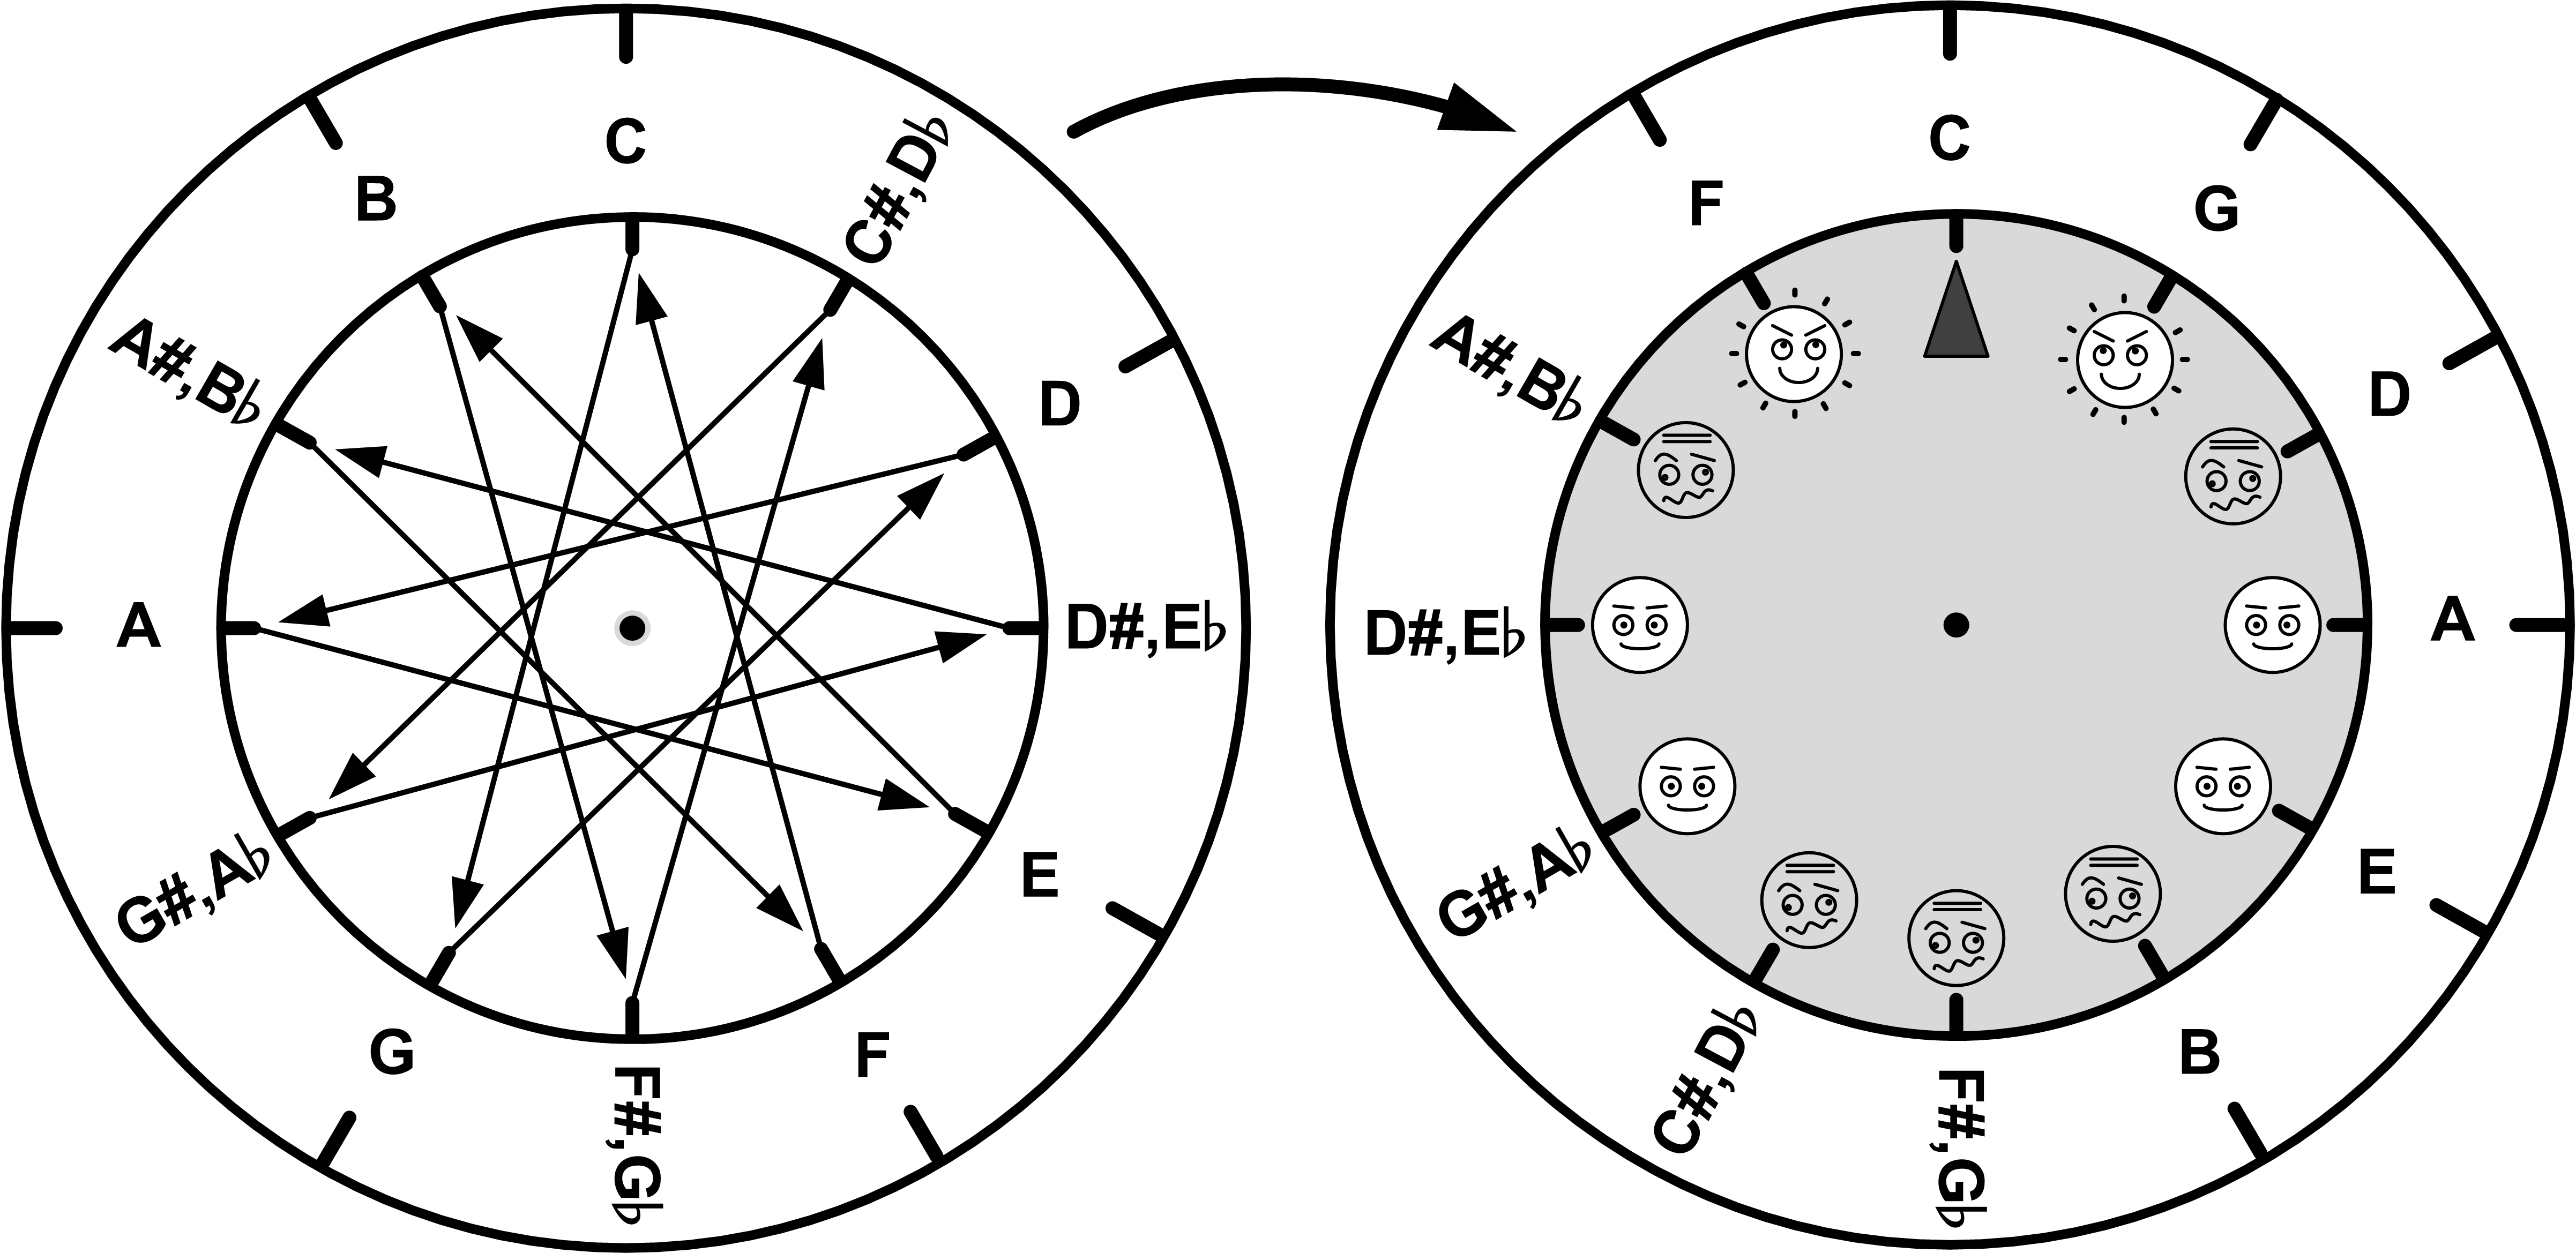
\includegraphics[scale=0.7]{fig/kvinto-kvarto/kons-rearrange} 
    \caption{Консонансы по соседству}\label{fig:harmony:kvinto-kvarto:kons-rearrange}
\end{figure} 

Теперь достаточно ткнуть в любую ноту на получившемся круге и узнать её совершенные консонансы: соседом против часовой стрелки будет совершенный консонанс на расстоянии 5 полутонов (чистая кварта), а по часовой --- консонанс на расстоянии 7 полутонов (чистая квинта). Например, возмьем ноту ЛЯ(A) и сразу определяем консонансы: РЕ(D) --- кварта от ЛЯ и МИ(E) --- квинта.

Обратите внимание на то, что среди переупорядоченных нот явно выделились две цепочки: цепочка нот без диезов и бемолей и цепочка нот со знаками альтерации. Конечно, это не случайность: ноты без диезов и бемолей --- это названия ступеней мажорного лада (а точнее --- тональность ДО-мажор). И само-собой, мажорный лад в своё время был сформирован с учетом расположения совершенных консонансов и вполне возможно, автор при этом глядел на полученный нами круг.

Итак, ноты тональности ДО-мажор выстроились в одну цепочку. При этом тоника --- ДО, идет в этой последовательности второй, если считать по часовой стрелке.

Таким образом упростилась задача определения нот для любой мажорной тональности: 
\begin{enumerate}
    \item нужно отметить тонику на круге и отступить от нее на один сектор против часовой стрелки;
    \item включая полученную ноту, двигаясь по часовой стрелке, отсчитать семь нот тональности.
\end{enumerate}

Например, требуется определить ноты тональности РЕ-мажор (см. рисунок \ref{fig:harmony:kvinto-kvarto:d-maj}). Отступаем от $D$ против часовой стрелки, а затем по часовой собираем 7 нот:
\[
    G\rightarrow 
    D\rightarrow 
    A\rightarrow 
    E\rightarrow 
    B\rightarrow 
    {F\sharp}\rightarrow
    {C\sharp}
\]

\begin{figure}[!ht]
    \centering
    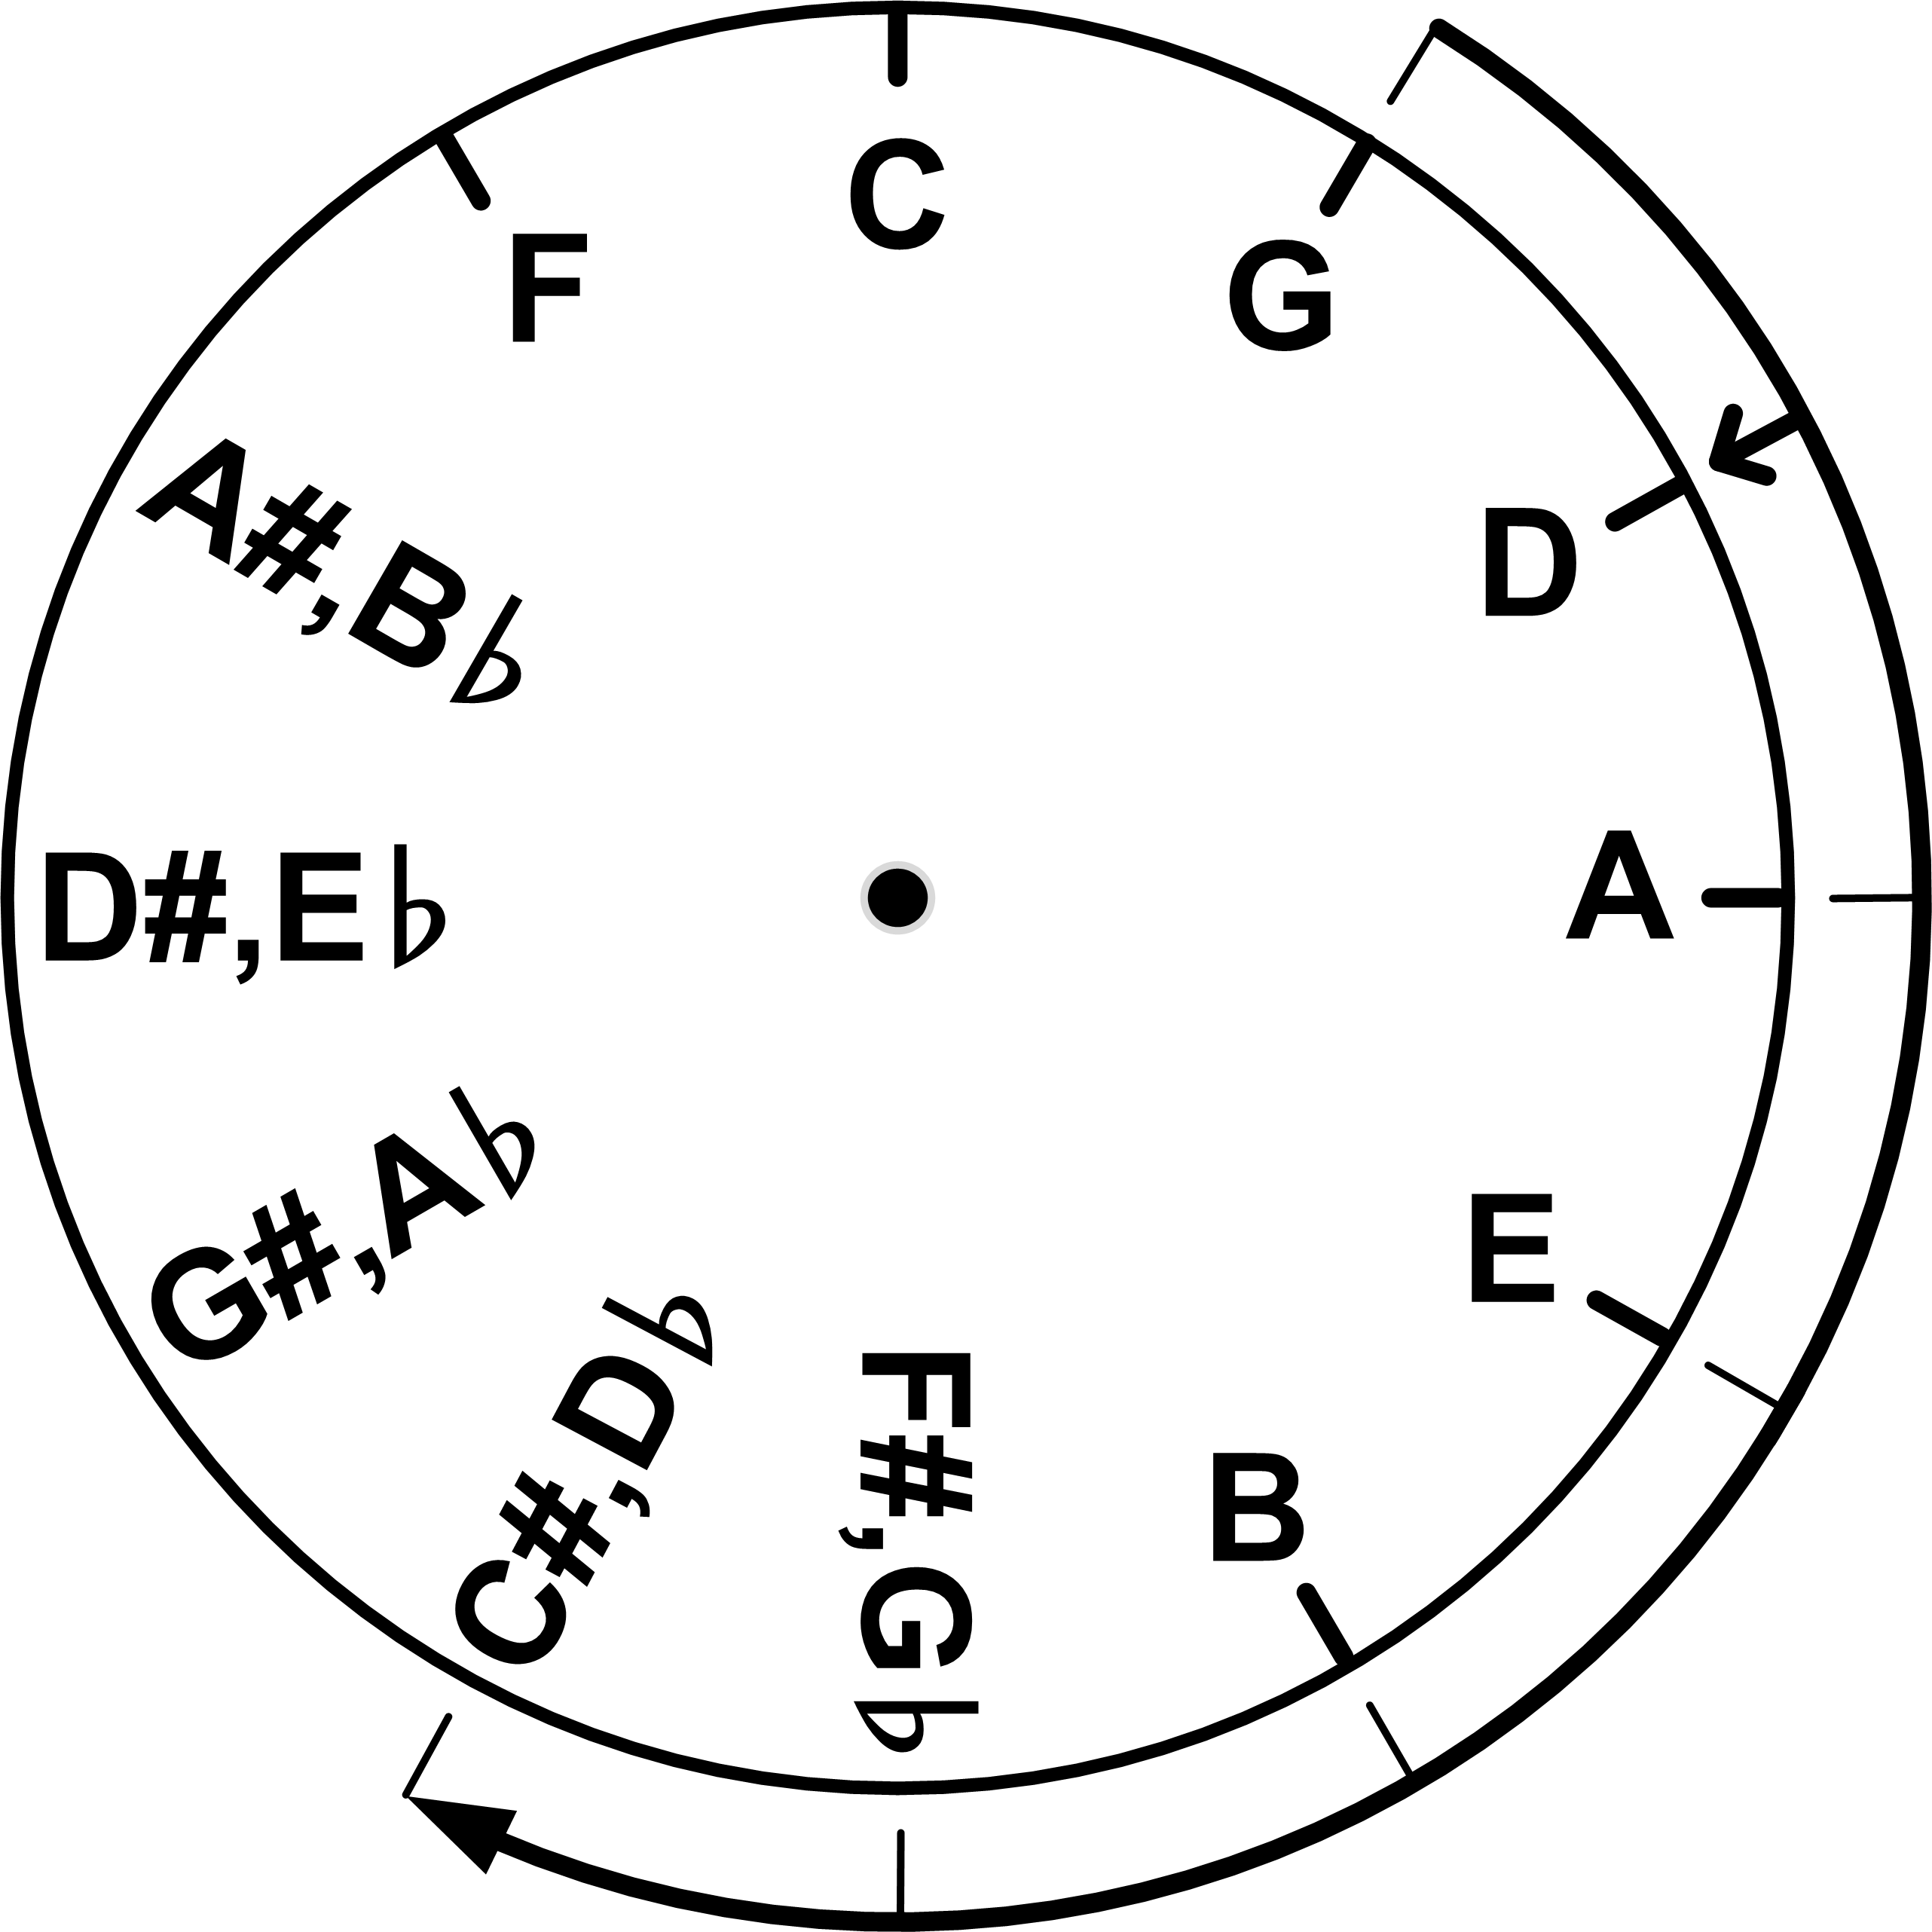
\includegraphics[scale=0.5]{fig/kvinto-kvarto/kvinto-kvarto-d-maj} 
    \caption{Ноты тональности D-maj}\label{fig:harmony:kvinto-kvarto:d-maj}
\end{figure} 

Естественно, что ноты по высоте пока не упорядочены, но это совсем несложно сделать, зная, что тоника внизу:
\[
    D\rightarrow 
    E\rightarrow 
    {F\sharp}\rightarrow
    G\rightarrow 
    A\rightarrow 
    B\rightarrow 
    {C\sharp}
\]
